\zotelo{../thesis.bib}

\chapter{Introduction}
\label{chap:intro}

A lot of astrophysics has to do with observing objects at various radiation
frequencies. Many objects are sources of high energy radiation, including but
not limited to pulsars, gamma-ray bursts, magnetars, super-massive black holes,
etc. In many of the objects, the spectrum is highly non-thermal, and the
radiation is produced by accelerated particles. The study of particle
acceleration and dissipation of other forms of energy into particle kinetic
energy is therefore vital in the study of high-energy astrophysics.

In many of the sources, the most notable source of energy for nonthermal
particles is the magnetic energy. In some sources such as pulsars, magnetic
field plays an intermediary role, acting as a channel that converts the
rotational energy of the pulsar ultimately into the particle energy, which then
is radiated away and produce the observed radio/X-ray/gamma ray emission. In
other sources such as magnetars it is the magnetic energy itself that is
directly converted to particle energy that is radiated.

% TODO: Go into more details, and mention past work
The dissipation of magnetic energy and acceleration of particles is a highly
nonlinear process, and very difficult to model directly. In the past people have
tried different methods. Some attempt to model the whole system by treating the
plasma as fluid, and use magnetohydrodynamics or force-free approximation. Some
isolate part of the system and study the detailed local evolution of
eletromagnetic fields. It is only recently that computational power has
increased to the level that we could attempt a first-principle direct simulation
of the system of interest.

This dissertation will be focusing on the physics of isolated neutron stars. In
the following sections we will examine the history and basic physics of
rotation-powered pulsars, and the exotic magnetars which have extremely high
magnetic field. Finally we will outline the chapters of the thesis.

\section{Pulsars}
\label{sec:intro-pulsars}

\subsection{Early Observations}

The first observational discovery of the rotation-powered pulsars (RPP) dates
back to late 1960s \citep{hewish_observation_1968}. In this paper a periodic
radio source was reported to be emitting regular pulsation at a frequency of
$81.5\,\mathrm{MHz}$, with a period of $1.337\,\mathrm{s}$ at extreme accuracy.
The pulse width of the object gives an upper bound on its physical size, which
should not exceed $4.8\times 10^3\,\mathrm{km}$. The extreme constancy of the
intrinsic period suggests that the source is a massive object, rather than some
astrophysical plasma configuration. It was therefore conjectured that this
pulsed radio emission was coming from a compact star: a white dwarf or a neutron
star; the extreme regular pulsation is a result of its rapid rotation
\citep{gold_rotating_1968}.

\begin{figure}[h]
  \centering
  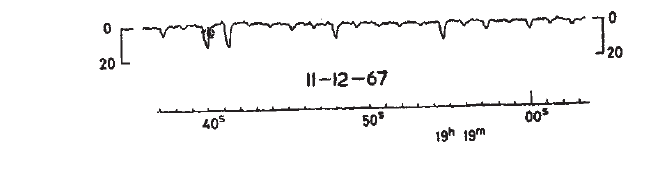
\includegraphics[width=0.6\textwidth]{pics/intro/pulses.png}
  \caption{A record of the pulsating radio source discovered in 1967
    \citep{hewish_observation_1968}}
  \label{fig:pulse}
\end{figure}

More pulsars were soon discovered, e.g.\ the Vela with a period of
$89\,\mathrm{ms}$ \citep{large_pulsar_1968} and the Crab with a period of
$33\,\mathrm{ms}$ \citep{lovelace_pulsar_1968}. Slowing down of the periods were
also discovered in the known pulsars. The spin-down luminosity can be easily
estimated given the period and period derivative of the pulsar:
\begin{equation}
  \label{eq:spindown-power}
  L = -I\Omega\dot{\Omega} = 4\pi^2 I\frac{\dot{P}}{P^3}
\end{equation}
which works out to be $\sim 10^{39}\,\mathrm{erg/s}$ for the Crab pulsar, which
has $P = 33\,\mathrm{ms}$ and $\dot{P} = 4.2\times 10^{-13}\,{s\;s^{-1}}$. This
matches the observed luminosity of the Crab nebula, and a model was soon
proposed by \citet{gold_rotating_1969} that gas was liberated from the star and
accelerated to relativistic energies, forming a corotating magnetosphere around
the star up to the radius where corotation speed becomes equal to the speed of
light, $R_\mathrm{LC} = c/\Omega$. This radius is called the light-cylinder
radius. In this model, the relativistic gas carry away most of the spin-down
luminosity, and make its contribution to the luminosity of the nebula.

The spin-down of the pulsar was typically modeled by a spinning magnetic dipole
in vacuum. A magnetic dipole of strength $\mu$ will lose energy at a rate:
\begin{equation}
  \label{eq:dipole-spin-down}
  L = \frac{2}{3}\frac{\mu^2\Omega^4}{c^3}
\end{equation}
therefore one can naively estimate the surface magnetic field by equating this
with the spin-down luminosity \eqref{eq:spindown-power}
\begin{equation}
  \label{eq:surface-B-field}
  B_0 = 3.2\times 10^{19}\sqrt{P \dot{P}}\,\mathrm{G}
\end{equation}

For typical pulsar parameters, this gives a polar magnetic field of the order
$\sim 10^{12}\,\mathrm{G}$. The strong magnetic field required rules out the
possibility of a white dwarf, and since then a rapid rotating neutron star has
been the standard model for a rotation-powered pulsar. Equation
\eqref{eq:surface-B-field} remains the standard formula for estimating the surface
magnetic field of a newly discovered pulsar.

\subsection{High-energy radiation from pulsars}
\label{sec:observ-high-energy}



\subsection{Theoretical models and problems}
\label{sec:intro-pulsar-theory}

Despite the success of a simple vacuum dipole model, it proves to be extremely
difficult to make a more detailed self-consistent model.

\section{Magnetars}
\label{sec:intro-magnetars}

\subsection{Observations}

\subsection{Theoretical Studies}
\label{sec:intro-magnetar-theory}


\section{This Dissertation}
\label{sec:intro-outline}

In this dissertation we will attempt to address the problem of particle
acceleration and global structure of the magnetosphere of pulsars and
magnetars.

Chapter \ref{chap:pic} will be devoted to a detailed introduction of the
particle-in-cell technique, which will be the basic numerical tool for our
study.

Chapter \ref{chap:polar-cap} will focus on a local study of the pulsar
polar cap. We will look at the region well within the pulsar magnetosphere, and
approximate the geometry as 1D. We will discuss implications of this
approximation, and what we can and can not learn from this local study.

Chapter \ref{chap:pulsar} will study the global pulsar magnetosphere, motivated
by the study of the polar cap particle acceleration.

Chapter \ref{chap:magnetar} will study the twisted magnetosphere of magnetars.

% Local Variables:
% TeX-master: "../thesis"
% zotero-collection: #("16" 0 2 (name "Thesis"))
% End:
